%---------------------------------------------------
\chapter{HTTP support} \label{sec:http}
%---------------------------------------------------

Similarly to OSC, several \faust architectures provide also HTTP support. This allows \faust applications to be remotely controlled from any Web browser using specific URLs. Moreover OSC and HTTPD can be freely combined.

While OSC support is installed by default when \faust is build, this is not the case for HTTP. That's because it depends on GNU \emph{libmicrohttpd} library which is usually not installed by default on the system. An additional \lstinline'make httpd' step is therefore required when compiling and installing \faust:
\begin{lstlisting}
make httpd
make
sudo make install
\end{lstlisting}
Note that \lstinline'make httpd' will fail if \emph{libmicrohttpd} is not available on the system.

The HTTP support can be activated using the \code{-httpd} option when building the audio application with the appropriate \code{faust2xxx} command. The following table (table \ref{tab:httparch}) lists \faust's architectures which provide HTTP support. 

\begin{table}[htdp]
\begin{center}
\begin{tabular}{rcc}
\hline
\bf{Audio system} 	& \bf{Environment} & \bf{HTTP support}	\\
\hline
%\OSTab{Linux} \\
%\multicolumn{3}{|l|}{Linux} \\
%\hline
\\
\emph{Linux}\\
Alsa  			& GTK, Qt, Console		& yes\\
Jack 			& GTK, Qt, Console		& yes\\
Netjack 			& GTK, Qt, Console & yes\\
PortAudio 		& GTK, Qt				& yes\\
%\hline
\\
\emph{Mac OS X} \\
%\hline
CoreAudio 		& Qt 			& yes\\
Jack 			& Qt, Console & yes\\
Netjack 			& Qt, Console & yes\\
PortAudio 		& Qt 			& yes\\
%\hline
\\
\emph{Windows} \\
%\hline
Jack 			& Qt, Console & yes\\
PortAudio 		& Qt 			& yes\\
%\hline
\hline
\end{tabular}
\end{center}
\caption{\faust architectures with HTTP support.}
\label{tab:httparch}
\end{table}


\section{A simple example}

To illustrate how HTTP support works let's reuse our previous \code{mix4.dsp} example, a very simplified monophonic audio mixer with 4 inputs and one output. For each input we have a mute button and a level slider:
\begin{lstlisting}
input(v) = vgroup("input %v", *(1-checkbox("mute")) 
         : *(vslider("level", 0, 0, 1, 0.01)));
process  = hgroup("mixer", par(i, 4, input(i)) :> _);
\end{lstlisting}

We are going to compile this example as a standalone Jack QT application with HTTP support using the command:
\begin{lstlisting}
faust2jaqt -httpd mix4.dsp
\end{lstlisting}
Th effect of the \code{-httpd} is to embed a small Web server into the application, which  purpose is to serve an HTML page representing its user interface. This page makes use of JavaScript and SVG and is quite similar to the native QT interface.

When we start the application from the command line:
\begin{lstlisting}
./mix4 
\end{lstlisting}
we get various information on the standard output, including:
\begin{lstlisting}
Faust httpd server version 0.72 is running on TCP port 5510
\end{lstlisting}

As we can see the embedded Web server is running by default on TCP port 5510. The entry point is \url{http://localhost:5510}. It can be open from any recent browser and it produces the page reproduced figure \ref{fig:mix4-http}.


\begin{figure}[h!]
  \centering
  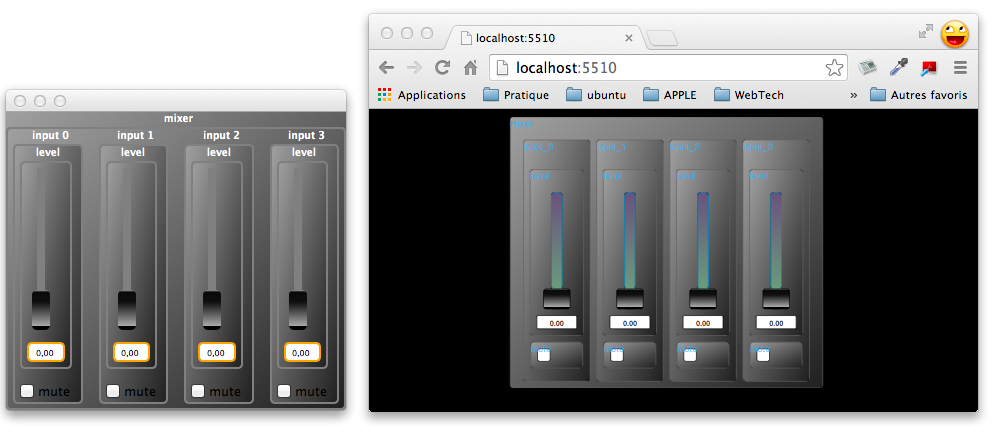
\includegraphics[scale=0.275]{images/mix4-http.png}
  \caption{User interface of mix4.dsp in a Web browser}   
  \label{fig:mix4-http}
\end{figure}

\section{JSON description of the user interface}
The communication between the application and the Web browser is based on several underlying URLs. The first one is \url{http://localhost:5510/JSON} that return a json description of the user interface of the application. This json description is used internally by the JavaScript code to build the graphical user interface. Here is (part of) the json returned by \code{mix4}:
\begin{lstlisting}
{
  "name": "mix4",
  "address": "YannAir.local",
  "port": "5511",
  "ui": [
    {
      "type": "hgroup",
      "label": "mixer",
      "items": [
        {
          "type": "vgroup",
          "label": "input_0",
          "items": [
            {
              "type": "vslider",
              "label": "level",
              "address": "/mixer/input_0/level",
              "init": "0", "min": "0", "max": "1", 
              "step": "0.01"
            },
            {
              "type": "checkbox",
              "label": "mute",
              "address": "/mixer/input_0/mute",
              "init": "0", "min": "0", "max": "0", 
              "step": "0"
            }
          ]
        },
        
        ...
        
      ]
    }
  ]
}
\end{lstlisting}

\section{Quering the state of the application}

Each widget has a unique "address" field that can be used to query its value. In our example here the level of the input 0 has the address \lstinline'/mixer/input_0/level'. The address can be used to forge an URL to get the value of the widget: \url{http://localhost:5510/mixer/input_0/level}, resulting in:
\begin{lstlisting}
/mixer/input_0/level 0.00000  
\end{lstlisting}

Multiple widgets can be query at once by using an address higher in the hierarchy. For example to get the values of the level and the mute state of input 0 we use \url{http://localhost:5510/mixer/input_0}, resulting in:
\begin{lstlisting}
/mixer/input_0/level 0.00000 
/mixer/input_0/mute  0.00000 
\end{lstlisting}

To get the all the values at once we simply use \url{http://localhost:5510/mixer}, resulting in:
\begin{lstlisting}
/mixer/input_0/level 0.00000 
/mixer/input_0/mute  0.00000 
/mixer/input_1/level 0.00000 
/mixer/input_1/mute  0.00000 
/mixer/input_2/level 0.00000 
/mixer/input_2/mute  0.00000 
/mixer/input_3/level 0.00000 
/mixer/input_3/mute  0.00000 
\end{lstlisting}

\section{Changing the value of a widget}

\begin{figure}[h!]
  \centering
  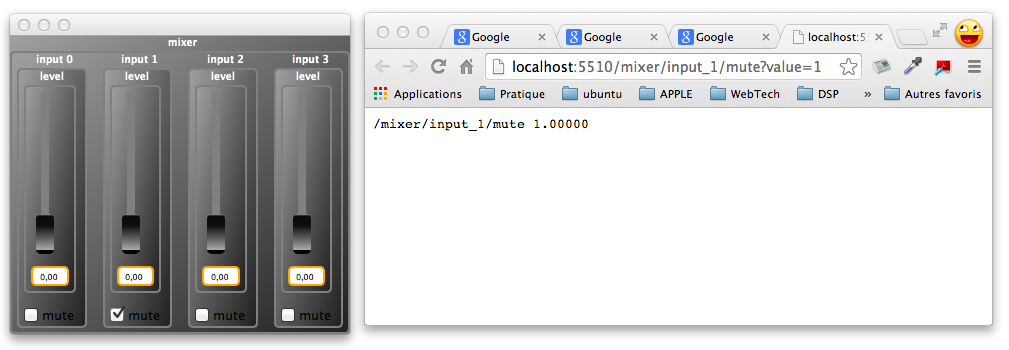
\includegraphics[scale=0.35]{images/mix4-http-mute.png}
  \caption{Muting input 1 by forging the appropriate URL}   
  \label{fig:mix4-http-mute}
\end{figure}

Let's say that we want to mute input 1 of our mixer. We can use for that purpose the URL \url{http://localhost:5510/mixer/input_1/mute?value=1} obtained by concatenating \url{?value=1} at the end of the widget URL. 

All widgets can be controlled similarly. For example \url{http://localhost:5510/mixer/input_3/level?value=0.7} will sets the input 3 level to 0.7.

\section{Proxy control access to the Web server}

A control application may want to access and control the running DSP using its Web server, but without using the delivered HTML page in a browser. Since the complete json can be retrieved,  control applications can purely be developed in C/C++, then build a \textit{proxy} version of the use interface, and set and get parameters using HTTP requests. 

This mode can be started dynamically using the \textit{ -server URL } parameter. Assuming an application with HTTP support is running remotely on the given URL, the control application will fetch its json description, use it to dynamically build the user interface, and allow to access the remote parameters.

\section{HTTP cheat sheet}
Here is a summary of the various URLs used to interact with the application's Web server.
\subsection*{Default ports}

\begin{tabular}{ll}
\lstinline'5510' & default TCP port used by the application's Web server\\
\lstinline'5511...' & alternative TCP ports
\end{tabular}

\subsection*{Command line options}

\begin{tabular}{rl}
\lstinline'-port' $n$ & set the TCP port number used by the application's Web server\\
\lstinline'-server' $URL$ & start a proxy control application accessing the remote application running on the given URL \\
\end{tabular}

\subsection*{URLs}

\begin{tabular}{ll}
\code{http://}\emph{host}\code{:}\emph{port} & the base URL to be used in proxy control access mode \\
\code{http://}\emph{host}\code{:}\emph{port}\code{/JSON} & get a json description of the user interface \\
\code{http://}\emph{host}\code{:}\emph{port}\code{/}\emph{address} & get the value of a widget or a group of widgets \\
\code{http://}\emph{host}\code{:}\emph{port}\code{/}\emph{address}\code{?value=}\emph{v} & set the value of a widget to $v$
\end{tabular}

\subsection*{JSON}
\subsubsection*{Top level}
The json describes the name, host and port of the application and a hierarchy of user interface items:
\begin{lstlisting}
{
  "name": <name>,
  "address": <host>,
  "port": <port>,
  "ui": [ <item> ]
}
\end{lstlisting}
An \code{<item>} is either a group (of items) or a widget.

\subsubsection*{Groups}
A group is essentially a list of items with a specific layout: 
\begin{lstlisting}
{
	"type": <type>,
	"label": <label>,
	"items": [ <item>, <item>,...]
}
\end{lstlisting}
The \code{<type>} defines the layout. It can be either \code{"vgroup"}, \code{"hgroup"} or \code{"tgroup"}

\subsubsection*{Widgets}
\begin{lstlisting}
{
	"type": <type>,
	"label": <label>,
	"address": <address>,
	"meta": [ { "key": "value"},... ],
	"init": <num>,
	"min": <num>,
	"max": <num>,
	"step": <num>
},
\end{lstlisting}
Widgets are the basic items of the user interface. They can be of different \code{<type>} : \code{"button"},  \code{"checkbox"}, \code{"nentry"}, \code{"vslider"}, \code{"hslider"}, \code{"vbargraph"} or \code{"hbargraph"}.



